\title{Physics 134 
\partition\
Physics Advanced Laboratory\\
\vspace{1ex}
Analysis of the Zeeman Effect on Mercury\\
\normalsize{Rick Ramirez}\\
\normalsize{Nathan Martinez}}

\date{Spring 2016}
\documentclass[12pt]{article}
\usepackage[margin=0.8in]{geometry}
\usepackage{amsmath, amssymb, enumerate, gensymb, wrapfig} %amssymb provides symbols for (integers, reals etc.)
\usepackage{verbatim} % Comment block.
\usepackage{pgfplots} % 3D plots
\pgfplotsset{compat=1.8}
\usepackage{mathrsfs} % provides cursive letters
\usepackage{caption, multirow}
\usepackage{booktabs}
\linespread{1.3}
\newcommand{\partition}{\rule{\linewidth}{0.8pt}}

% my own titles
\makeatletter
\renewcommand{\maketitle}{
\begin{center}
\@date \hfill  \@author\\
{\Large \textsc{\@title}}
\partition\\
\end{center}
}
\usepackage{tikz}

%%%----------%%%----------%%%----------%%%----------%%%----------%%%
%%%----------%%%----------%%%----------%%%----------%%%----------%%%

\begin{document}
\maketitle
\linespread{1.5}
\abstract{
\noindent
By applying a magnetic field to mercury, we were able to measure the splitting of the energy levels of. The measurements allowed us to calculate the value of the Bohr magneton. For pi-transitions, the measured value is $\mu_B = 5.62 \pm 0.20 \times 10^{-05} \text{eV T}^{-1}$ and $\mu_B = 5.39 \pm 0.27 \times 10^{-05} \text{eV T}^{-1}$. For sigma-transitions, $\mu_B = 5.18 \pm 0.40 \times 10^{-05} \text{eV T}^{-1}$, and $\mu_B = 5.80 \pm 0.61 \times 10^{-05} \text{eV T}^{-1}$.
} 


\section{Introduction}

An atom that is placed in a uniform magnetic field will exhibit a splitting of its energy levels. For a magnetic field applied to the z-direction, the perturbing Hamiltonian takes the form
\begin{equation}
H' = -(\mu_l + \mu_s) \cdot \bf{B}_{ext}, 
\end{equation}\label{eq:H}
where $\mu_s = -\frac{e}{m}\bf{S}$ and $\mu_l = -\frac{e}{2m}\bf{L}$ are the magnetic dipole moments associated with an electron's spin and orbital motion respectively. The role of the Zeeman effect depends on the strength of the external field in relation to the internal field. The internal field is produced by spin-orbit coupling and relativistic corrections of the electron \cite{Sakurai}, and gives rise to fine structure splitting. If the internal field is the dominating term, then fine structure splitting prevails, and $H'$ can be treated as a small perturbation. At the other extreme, If the external field dominates, then the fine structure contribution becomes the perturbing term. The intermediate zone, where Zeeman and fine structure are comparable to each other, requires a denationalization of the relevant portion of the Hamiltonian to determine the nature of the splitting. A further shift in energy is caused by interactions between the magnetic moments of the nucleus and electron and is referred to as hyperfine splitting. 
\subsection{Weak External Field}
If the external field is much less than the internal field, then spin-orbit interactions dominate, and the Hamiltonian no longer commutes with $\bf{L}$ and $\bf{S}$. The effect is that both $\bf{L}$ and $\bf{S}$ are not separately conserved. As a result, the state of the system can be described as 
\begin{equation}
|n, l, j, m_j\rangle,
\end{equation}\label{eq:state}
neglecting $m_l$, and $m_s$. The first order correction to the energy can be found by considering the time independent Schridinger equation
\begin{equation}
H|\psi\rangle = E|\psi\rangle,
\end{equation}
where the Hamiltonian is that of Eq.\ref{eq:H} acting on the state in Eq.2. Taking the inner product with the eigenbra $\langle n, l, j, m_j|$, we have
\begin{equation}
E = \langle n, l, j, m_j|H|n, l, j, m_j\rangle = \frac{e}{2m}\bf{B}_{ext}\langle \bf{L} + 2\bf{S}\rangle
\end{equation}
where $\bf{L} + 2\bf{S} = \bf{J} + \bf{S}$. The expectation value of $\bf{S}$ is unknown, however the total angular momentum is constant with $\bf{L}$ and $\bf{S}$ precessing  about fixed $\bf{J}$. \cite{Griffiths} If the average value of $\bf{S}$ is taken to be the projection along $\bf{J}$, then
\begin{equation}
\bf{S}_{avg} = \frac{(\bf{S} \cdot \bf{J})}{J^2}\bf{J}\:.
\end{equation}
\noindent
The square of the orbital angular momentum of the system can be expressed as 
\begin{equation}
L^2 = J^2 + S^2 -2\bf{J}\cdot \bf{S}\:,
\end{equation}
allowing $\bf{S} \cdot \bf{J}$ to be expressed in terms of $J^2$, $S^2$ and $L^2$; each of which have known eigenvalues. That is 
\begin{equation}
\textbf{S} \cdot \textbf{J} = \frac{1}{2}(J^2 + S^2 + L^2) = \frac{\hbar}{2}[j(j+1) + s(s+1) + l(l+1)]\:.
\end{equation}
The expectation value of Eq.4 can then be expressed as
\begin{equation}
\begin{split}
\langle \textbf{L} + 2\textbf{S}\rangle = \langle \textbf{J} + \frac{(\textbf{S} \cdot \textbf{J})}{J^2}\textbf{J}\rangle = \left[ 1+ \frac{j(j+1) + s(s+1) + l(l+1)}{2j(j+1)} \right]\langle \textbf{J}\rangle
\end{split}\:,
\end{equation}
where the term in the square brackets is the Lande g-factor. Therefore, the first order correction to the energy takes the form
\begin{equation}
E' = \frac{e\hbar}{2m} \:g\: \text{B}_{ext}
\end{equation}

\subsection{Zeeman effect of mercury}
Mercury has an atomic number of $Z=80$, with an electron configuration of 
\begin{equation}
[\text{Xe}] = 4f^{14}5d^{10}6s^2\:.
\end{equation}
When gaseous mercury is subjected to an electrical discharge, a $6s$ electrons can be excited into the $7s$ orbital. As the electron de-excites to its original state, it first transitions to a $6p$ orbital before returning $6s$. The de-excitation process can be written as
\begin{equation}
{}^3S_1 \longrightarrow {}^3P_2 \longrightarrow {}^1S_0\:,
\end{equation}
where the superscript corresponds spin, the letter corresponds to orbital angular momentum, and the subscript corresponds to total angular momentum. For the transition, ${}^3S_1 \longrightarrow {}^3P_2$, a photon of $\lambda = 546.07$nm is emitted. The total angular momentum quantum number of the two electrons in the initial state is $J=1$, and for the final state, $J=2$. The z-projection can range in values from $-j\leq m_j \leq j$ resulting in $2j+1$ possible transitions. With the stipulation that $\Delta m_j = 0,\pm 1$, the possible transitions diminish from 15 to only 9. \cite{manual} If the photons produced by a transition are observed perpendicular from the source, transitions resulting from $\Delta m_j = 0$ will be polarized parallel to the magnetic field, while $\Delta m_j = \pm 1$ will be polarized perpendicular to the field. Using Eq.9, the shift in energy can be rewritten for a transition between two orbitals as
\begin{equation}
E' = [g_im_{j_i} - g_f m_{j_f}]\mu_B B_{ext}\:,
\end{equation}
where $\mu_B = \frac{e\hbar}{2m} = 5.788 381 8066(38)\times 10^{-5}\textit{eVT}^{-1}$ \cite{pdg} is the Bohr magneton, and g is the Lande g-factor for the initial and final state, and . The 9 possible transitions and their shift in energy are depicted Fig.\ref{fig:transitions}. Depending on the transition involved, the shift in energy level from the unperturbed system can take values of -2, -3/2,-1/2, -1, 0, 1/2, 1, 3/2, or 2 times the energy of the unperturbed case.  Light observed using the configuration outlined in section 2 will consist of a series of rings as shown in Fig.\ref{fig:90}. As the magnetic field increases, the splitting of an energy level corresponds to a splitting on the Zeeman rings. The change in energy is related to the angular diameter of the rings by
\begin{equation}
\bar{E}[(\theta_p^a)^2 - (\theta_p^b)^2] = 2(E_a - E_b)\:,\quad \cite{manual}
\end{equation}
where $\bar{E}$ is the energy associated with $\lambda = 246.07$nm and p is the ring index.
\begin{figure}[h!]\centering
 \quad \includegraphics[width=1\textwidth]{90}
\caption{Image of Zeeman rings for a $\pi$ transition of mercury. The image on the left is light produced by an unperturbed transition, while the image on the right is the result of exposing the mercury to a magnetic field of 6.9KG.}
\label{fig:90}
\end{figure}
\begin{figure}[h!]\centering
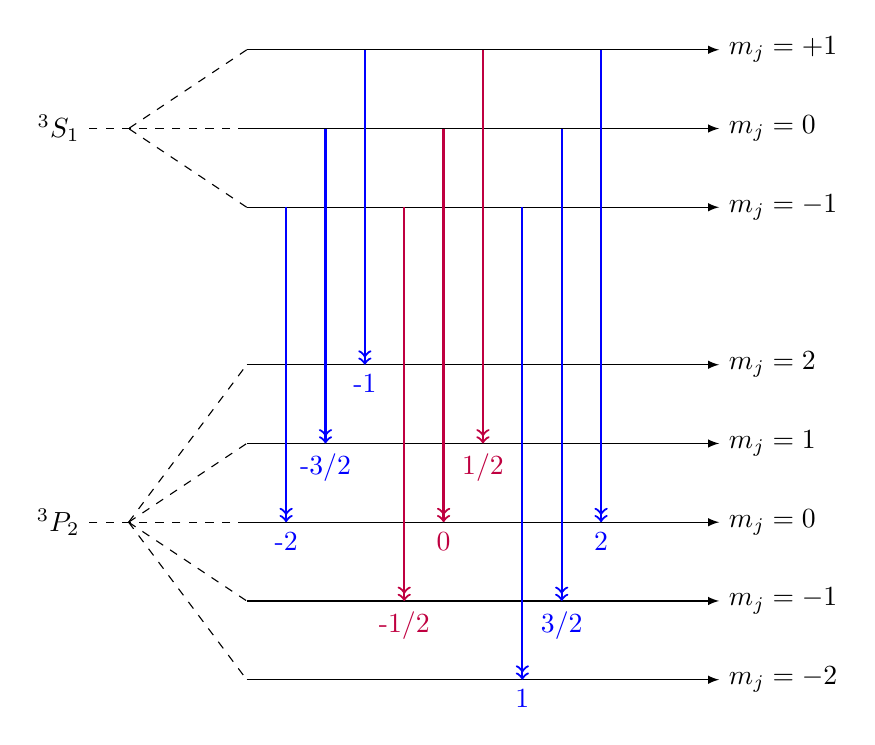
\begin{tikzpicture}[scale= 1]
  \draw[-latex] (-3,3) -- (3,3) node[right] {$m_j = +1$};
  \draw[-latex] (-3,2) -- (3,2) node[right] {$m_j = 0$};
  \draw[-latex] (-3,1) -- (3,1) node[right] {$m_j = -1$};
  \draw[-latex] (-3,-1) -- (3,-1) node[right] {$m_j = 2$};
  \draw[-latex] (-3,-2) -- (3,-2) node[right] {$m_j = 1$};
  \draw[-latex] (-3,-3) -- (3,-3) node[right] {$m_j = 0$};
  \draw[-latex] (-3,-4) -- (3,-4) node[right] {$m_j = -1$};
  \draw[-latex] (-3,-5) -- (3,-5) node[right] {$m_j = -2$};
      
  \draw[dashed] (-3,3) -- (-4.5,2) node[left] {};
  \draw[dashed] (-3,2) -- (-5,2) node[left] {$^3S_1$};
  \draw[dashed] (-3,1) -- (-4.5,2) node[left] {};
  
  \draw[dashed] (-4.5,-3)--(-3,-1) node[left] {};
  \draw[dashed] (-4.5,-3)--(-3,-2) node[left] {};
  \draw[dashed] (-3,-3)--(-5,-3) node[left] {$^3P_2$};
  \draw[dashed] (-4.5,-3)--(-3,-4) node[left] {};
  \draw[dashed] (-4.5,-3)--(-3,-5) node[left] {};
  
  \draw[thick, color=blue, ->>] (-2.5,1) -- (-2.5,-3) node[below] {-2};
  \draw[ thick, color=blue, ->>] (-2,2) -- (-2,-2) node[below] {-3/2};
  \draw[ thick, color=blue, ->>] (-1.5,3) -- (-1.5,-1) node[below] {-1};
  
  \draw[ thick, color=purple, ->>] (-1,1) -- (-1,-4) node[below] {-1/2};
  \draw[ thick, color=purple, ->>] (-0.5,2) -- (-0.5,-3) node[below] {0};
  \draw[ thick, color=purple, ->>] (0,3) -- (0,-2) node[below] {1/2};
  
  \draw[thick, color=blue, ->>] (0.5,1) -- (0.5,-5) node[below] {1};
  \draw[ thick, color=blue, ->>] (1,2) -- (1,-4) node[below] {3/2};
  \draw[ thick, color=blue, ->>] (1.5,3) -- (1.5,-3) node[below] {2};
\end{tikzpicture}
\caption{9 possible transitions between $^3S_1$ and $^3P_2$. Adapted from \cite{manual,Melissinos}}
\label{fig:transitions}
\end{figure}\\
\newpage


\section{Experimental Setup}
The apparatus consists of a light source in the form of a hollow-cathode mercury discharge tube powered by an alternating current. The tube is immediately followed by a 0.4mm diameter aperture. The aperture ensures that only light from center of the magnetic field is exposed to the optics. Following the light source is a condenser consisting of a bi-convex lens with a focal length of 150mm, and is placed roughly 300mm from the source. The image produced has unity magnification at about 300mm downstream.
\begin{figure}[h!]\centering
 \quad \includegraphics[width=0.8\textwidth]{optical}
\caption{Layout of source and optical elements. S: source, CL: condenser lens, F: interference filter, FP: Fabry-Perot interferometer, LP: linear polarizer, A: aperture, OL: camera objective lense, CCD: charge coupled device. Image taken from \cite{manual}}
\label{fig:optical}
\end{figure}
Following the condenser is a polarizer with an adjustable orientation. Light that enters the polarizer from a direction perpendicular to the direction of the magnetic field will be linearly polarized.  The polarizer is followed by a interference filter. The spectrum of mercury is extremely complicated, and the interference filter allows only specific wavelength to be selected; $\bar{\lambda} = 546.07$nm in our case. Next is a Fabry-Perot interferometer consisting of two optical flats separated by a distance $t = 6.499$mm. Each flat is silvered with 90\% reflectivity. The final optical element consists of a $f = 135$mm focal length lens attached to an astronomical CCD camera, which is immediately preceded by a adjustable aperture. The lens is focused to infinity so that incoming parallel rays making an angle $\theta$ with the optical axis are focused at a distance $f\theta$ from the center of the image. The CCD camera contains an array of $510\times 765$ pixels, each with an area of $81\mu m^2$. A schematic of the source and optical elements can be seen in Fig.\ref{fig:optical}.\\

\noindent
The magnetic field applied to the mercury tube is produced by an iron-core electromagnet arranged in a horseshoe configuration, and is powered by a KEPCO power supply that can furnish a maximum of 80 volts and 2.0 Amperes. The strength of the field is measured with the axial probe of a LakeShore 425 gaussmeter. The axial probe has an operating temperature range of \cite{gaussmeter} $0\degree$C to $75\degree$C.
\section{Procedure}
Each of the optical elements were placed approximately 11cm above the table to ensure that only photons exposed to the magnet field were recorded. To ensure that none of the components connected to the mercury tube were damaged, the autotransformer was set to operate at 40 volts. Two sheets of paper were placed around the portion of the tube not exposed to the magnetic field. This further ensured that the light emitted will exhibit Zeeman splitting. The aperture that precedes the camera lens was adjusted to a diameter of 4.75cm.\\

\noindent
With the polarizer set to $0\degree$ and  the camera set to 0.5 second exposure times, the rotating platform on which the interference filter sits was adjusted until the sharpness of the rings was maximized. This was followed by a adjustment of the objective lens until the rings were as distinct as possible. With the magnet field off, the rings were exposed to the lens in 20 second exposure times. An analysis of the data can be seen in section 4.\\

\noindent
With the polarizer still set to $0\degree$, the KEPCO power supply was set to its maximum voltage of 80 volts with the current set to zero Amperes. The current was then increased in steps of 0.1 Amperes until it reached its maximum allowed value. An image of the Zeeman rings was recorded in 20 second exposure times for each increase in current. The magnet field at each interval was measured with the axial probe of the gaussmeter, and recorded. The tip of the probe was placed perpendicular to the direction of the magnetic field and adjusted until the largest stable measurement was obtained.\\

\noindent
When the maximum current was reached, the power supply was shut off and the dials set back to zero. The polarizer was then set to $90\degree$, and the process was repeated.


\section{Analysis}
\subsection{Zeeman Ring Linearity}
With the camera lens focused at infinity and a focal length of $f = 135$mm,  incoming rays parallel to the optical axis are focused at a distance $f\theta$ from the center of the image. The angular radius of the corresponding Zeeman ring is then $\theta_P = \tan^{-1}\left(\frac{d}{f}\right)$ where d is the radius of the ring. as shown in Fig.\ref{fig:incoming}.


\begin{figure}[h]\centering
\begin{tikzpicture}[scale=0.8]
  \draw[-latex] (-4,0) -- (4,0) node[right] {$x$};
  \draw[dashed] (3,2.5)--(-0,2.5) node[left] {};
  \draw[] (3,2.5)--(3,2.5) node[right] {incoming photon};
  \draw[dashed] (-3,0)--(-0,2.5) node[left] {};
  \draw[] (-2.4,0.2)--(-2.4,0.2) node[right] {$\theta$};  
  \draw[-latex] (0,-0.2) -- (0,3.2) node[above] {d};  
  \foreach \x/\xtext in {-3/f}
    \draw[shift={(\x,0)}] (0pt,0pt) -- (0pt,-8pt) node[below] {$\xtext$};
  \foreach \y/\ytext in {2.5/n, 2/, 1.5/, 1/}
    \draw[shift={(0,\y)}] (2pt,0pt) -- (-2pt,0pt) node[left] {$\ytext$};  
\end{tikzpicture}
\caption{Depiction of a photon incident on the camera.}
\label{fig:incoming}
\end{figure}
\noindent
Because rays of light that make it to the camera have unity transmission at angles given by 
\begin{equation}
 \theta^2 = \frac{\lambda}{t}(p - e(\lambda))\:,
 \end{equation} 
\noindent
the slope of the angular radius as a function of Zeeman ring is $\lambda/t = 8.40\times 10^{-5}$. A linear fit of the data in Table \ref{tab:linearset} produces 6 degrees of freedom and a goodness of fit value of 1.74. The slope of the fit in Fig.\ref{fig:zring} is measured to be $8.43(8)\times 10^{-5}$ with a confidence level of 94.22\%.\\

\begin{table}[h!]\centering
\begin{tabular}{ |p{1.5cm}|p{2.5cm}|p{2.5cm}|}
 \hline
  Ring P & $\theta^2$ (radians) & error \\
 \hline
 0 &  3.84E-05 & 1.00E-06\\
 \hline
 1 &  1.23E-04 & 1.00E-06\\
 \hline
 2 &  2.07E-04 & 1.00E-06\\
 \hline
 3 &  2.91E-04 & 1.00E-06\\
 \hline
 4 &  3.76E-04& 1.00E-06\\
 \hline
 5 &  4.61E-04 & 1.00E-06\\
 \hline
 6 &  5.44E-04 & 1.00E-06\\
 \hline
 7 &  6.28E-04 & 1.00E-06\\
 \hline
\end{tabular}
\def\sym#1{\ifmmode^{#1}\else\(^{#1}\)\fi}
\caption{Angular diameter of Zeeman rings with zero magnetic field, with corresponding ring index.}
\label{tab:linearset}
\end{table}

\begin{figure}[h!]\centering
 \quad \includegraphics[width=0.8\textwidth]{zring}
\caption{Linear fit of angular radius of Zeeman rings with magnetic field off. }
\label{fig:zring}
\end{figure}

\newpage
\subsection{Pi Transitions}
With the polarizer set to $90\degree$, the splitting of the first ring, p = 1, was monitored by taking the difference of the angular radius between the center and left peak followed by the difference between the center and right peak as shown in Fig.\ref{fig:90split}.

\begin{figure}[h!]\centering
 \quad \includegraphics[width=01\textwidth]{90split}
\caption{Plot of Zeeman rings as a function of intensity for $\pi$ transitions. The image on the top is the unperturbed case, while the bottom image corresponds to a magnetic field of 6.98KG. For the bottom image, the first largest peak on the left and right from the center correspond to p=1. The two smaller peaks on either side correspond to the splitting of the energy level. }
\label{fig:90split}
\end{figure}
\begin{figure}[h!]\centering
 \quad \includegraphics[width=1\textwidth]{90deg}
\caption{Shift in energy as a function of magnetic field for $\pi$ transitions. Both images correspond to a mapping of ring index p=1. The image on the left corresponds to the left peak of Fig.\ref{fig:90split}, while the image on the right corresponds to the right peak. All data can be seen in the appendix.}
\label{fig:90deg}
\end{figure}
\noindent
Using Eq.13 and Eq.12, the shift in energy in electron volts can be measured as a function of magnetic field in Tesla as shown in Fig.\ref{fig:90deg}. As the magnetic field increases, there is an increased spreading of the main peak into three distinct peaks. From Eq.12, we see that the slope of a linear fit to the data corresponds to the value of Bohr magneton. The results of the fit  for $m_j = +1$  and $m_j = -1$ are summarized in Table \ref{tab:m1}. The error on the measurement was found by considering the resolution power \cite{manual} ($\Delta \lambda / \lambda = 1.4\times 10^{-6}$) of the apparatus outlined in section 2. The error was adjusted by hand until the value of $\chi^2$ approached an appropriate value for the particular degree of freedom.

\begin{table}[h!]\centering
\begin{tabular}{|p{3cm} |p{3cm}|p{2cm}|p{2.5cm}|p{3.25cm}|}
 \hline
 &  $\mu_B$ (eV T${}^{-1}$)& DOF & $\chi^2$ & Confidence level \\
 \hline
$m_j = +1$ &  $5.62 \pm 0.20 \times 10^{-5}$ &  14 & 6.95 & 93.65\%\\
 \hline
$m_j = -1$ & $5.39 \pm 0.23 \times 10^{-5}$ & 13  & 6.29 & 93.48\%\\
 \hline
\end{tabular}
\def\sym#1{\ifmmode^{#1}\else\(^{#1}\)\fi}
\caption{Linear fit for the shift in energy of $\pi$ transitions as a function of magnetic field.}
\label{tab:m1}
\end{table}
%%%%%%%%%%%%%%%%%%%%%%%%%%%%%%%%%%%%%%%%%%%%%%%%%%%%%%%%%%%%%%%%%%%%%%%%%%%%%%


\subsection{Sigma Transitions}
Setting the polarizer to $0\degree$ allows for the transmission of $\Delta m_j = \pm 1$ photons. These transitions correspond to triplet configurations whose angular spacing is too fine to be resolved by the apparatus. This results in the three distinct lines in Fig.\ref{fig:transitions} forming two broad peaks as shown in Fig.\ref{fig:0split}. The average shift in energy for the two peaks will be $\pm 1.25 \mu_B B$ \cite{manual}. Because the center of the plot becomes extremely distorted, the Zeeman ring p=2 was chosen to be monitored. A summary of the results of a linear fit can be found in Table \ref{tab:m2}. 


\begin{figure}[h!]\centering
 \quad \includegraphics[width=01\textwidth]{0split}
\caption{Plot of Zeeman rings as a function of intensity for $\sigma$ transitions. The top image corresponds to zero magnetic field and the bottom image corresponds to a magnetic field of 8.94KG.  }
\label{fig:0split}
\end{figure}

\begin{figure}[h!]\centering
 \quad \includegraphics[width=01\textwidth]{0}
\caption{Shift in energy as a function of magnetic field for $\pi$ transitions. Both images correspond to a mapping of ring index p=2. The image on the left corresponds to the left peak from the center of p=2 of Fig.\ref{fig:0split}, while the image on the right corresponds to the right peak. }
\label{fig:0}
\end{figure}

\begin{table}[h!]\centering
\begin{tabular}{|p{4cm} |p{3cm}|p{2cm}|p{2.5cm}|p{3.25cm}|}
 \hline
 &  $\mu_B$ (eV T${}^{-1}$)& DOF & $\chi^2$ & Confidence level \\
 \hline
$\langle \delta E\rangle = +1.25\mu_BB$ &  $5.18 \pm 0.40 \times 10^{-5}$ &  14 & 7.00 & 93.44\%\\
 \hline
$\langle \delta E\rangle = -1.25\mu_BB$ & $5.80 \pm 0.61 \times 10^{-5}$ & 13  & 10.77 & 63.05\%\\
 \hline
\end{tabular}
\def\sym#1{\ifmmode^{#1}\else\(^{#1}\)\fi}
\caption{Linear fit for the shift in energy of $\sigma$ transitions as a function of magnetic field.}
\label{tab:m2}
\end{table}



\section{Conclusion}
By subject excited mercury atoms to a range of magnetic field intensities, we were able to track the shift in energy levels for transitions between the ${}^3S_1$ and ${}^3P_2$ orbitals. A linear fit to four sets of data produced values for the Bohr magneton of $\mu_B = 5.62 \pm 0.20 \times 10^{-05} \text{eV T}^{-1}$ and $\mu_B = 5.39 \pm 0.27 \times 10^{-05} \text{eV T}^{-1}$ for pi-transitions. For sigma-transitions, $\mu_B = 5.18 \pm 0.40 \times 10^{-05} \text{eV T}^{-1}$, and $\mu_B = 5.80 \pm 0.61 \times 10^{-05} \text{eV T}^{-1}$.
\\\\\\\\\\\\\\\\\\\\\



\begin{thebibliography}{9}

\bibitem{manual}
Physics 134 Lab Manual. Spring 2016 (Unpublished)

\bibitem{gaussmeter}
KEPCO. inc
\textit{User’s Manual Model 425 Gaussmeter}. 

\bibitem{pdg}
P.J. Mohr et al. \textit{Particle Data Group}\\
http://pdg.lbl.gov/2014/reviews/rpp2014-rev-phys-constants.pdf

\bibitem{Griffiths}
David J. Griffiths.
\textit{Introduction to Quantum Mechanics (2nd Edition)}. Pearson Prentice Hall (2004), ISBN-13: 978-0131118928

\bibitem{Sakurai}
J. J. Sakurai.
\textit{Modern Quantum Mechanics (2nd Edition)}. Pearson Prentice Hall (2010),  ISBN-13: 978-0805382914

\bibitem{Melissinos}
Adrian C. Melissinos.
\textit{Experiments in Modern Physics, Second Edition}.Academic Press (2003),  ISBN-13: 978-0124898516
\end{thebibliography}

\newpage
\section{Appendix}
For $\lambda = 546.07$nm, $\bar{E} = 2.27048$ eV. The error on the magnetic field measurements were taken to be $5.00\times 10^{-4}\: T^{-1}$.


\begin{table}[h!]\centering
\begin{tabular}{ |p{3cm}|p{3cm}||p{3cm}|p{3cm}|}
 \hline
  B ($T^{-1}$)& $\bar{E} * \delta\theta_{p=1} $ (eV)& B ($T^{-1}$) & $\bar{E} *\delta\theta_{p=1}$ (eV) \\
 \hline
3.15E-01&	3.92E-05&	3.88E-01&	3.67E-05\\
3.88E-01&	3.99E-05&	4.46E-01&	4.42E-05\\
4.46E-01&	3.99E-05&	5.19E-01&	4.50E-05\\
5.19E-01&	4.99E-05&	6.16E-01&	4.98E-05\\
6.16E-01&	5.44E-05&	6.98E-01&	5.81E-05\\
6.98E-01&	6.36E-05&	7.48E-01&	6.16E-05\\
7.48E-01&	6.66E-05&	8.27E-01&	8.15E-05\\
8.27E-01&	7.34E-05&	8.94E-01&	7.74E-05\\
9.04E-01&	7.74E-05&	9.75E-01&	8.52E-05\\
9.78E-01&	8.28E-05&	1.05E+00&	9.15E-05\\
1.05E+00&	8.81E-05&	1.12E+00&	9.78E-05\\
1.13E+00&	9.35E-05&	1.20E+00&	1.04E-04\\
1.20E+00&	9.88E-05&	1.27E+00&	1.10E-04\\
1.28E+00&	1.04E-04&	1.35E+00&	1.17E-04\\
1.35E+00&	1.10E-04&	1.42E+00&	1.23E-04\\
1.15E+00&	7.75E-05& &\\
\hline
$\bar{E} * \delta\theta_p$ Error: & 3.00E-06 & $\bar{E} * \delta\theta_p$ Error:  & 3.50E-06\\
\hline
\end{tabular}
\def\sym#1{\ifmmode^{#1}\else\(^{#1}\)\fi}
\caption{Data collected for $\pi$ transitions. The left two columns correspond the $m_j = +1$ transitions and the right two columns correspond to $m_j = -1$ transitions.}
\label{tab:pitrans}
\end{table}

\begin{table}[h!]\centering
\begin{tabular}{ |p{2.5cm}|p{2.5cm}||p{2.5cm}|p{2.5cm}|p{2.5cm}|p{2.5cm}|}
 \hline
  B ($T^{-1}$)& $\bar{E} * \delta\theta_{p=2}$ (eV)& B ($T^{-1}$) & $\bar{E} * \delta\theta_{p=2}$ (eV)\\
 \hline
3.03E-01&	1.91E-05&	3.81E-01&	1.76E-05 \\
3.81E-01&	2.05E-05&	4.76E-01&	3.05E-05\\
4.76E-01&	2.51E-05&	5.36E-01&	3.29E-05\\
5.36E-01&	2.62E-05&	6.14E-01&	3.92E-05\\
6.14E-01&	2.95E-05&	6.90E-01&	3.85E-05\\
6.90E-01&	3.81E-05&	7.70E-01&	4.43E-05\\
7.70E-01&	3.81E-05&	8.01E-01&	4.43E-05\\
8.01E-01&	4.51E-05&	8.72E-01&	4.63E-05\\
8.72E-01&	4.99E-05&	9.45E-01&	5.04E-05\\
9.45E-01&	4.99E-05&	9.92E-01&	5.54E-05\\
9.92E-01&	5.47E-05&	1.02E+00&	5.91E-05\\
1.02E+00&	5.47E-05&	1.07E+00&	6.14E-05\\
1.07E+00&	5.84E-05&	1.09E+00&	6.01E-05\\
1.09E+00&	6.13E-05&	1.09E+00&	6.07E-05\\
1.09E+00&	6.13E-05&	1.12E+00&	6.23E-05\\
1.12E+00&	6.13E-05&		&\\
\hline
$\bar{E} * \delta\theta_p$ Error: & 6.2E-06 & $\bar{E} * \delta\theta_p$ Error:  & 6.50E-06\\
\hline
\end{tabular}
\def\sym#1{\ifmmode^{#1}\else\(^{#1}\)\fi}
\caption{Data collected for $\sigma$ transitions. The left two columns correspond the $\langle\delta E\rangle = +1.25 \mu_BB$ transitions and the right two columns correspond to $\langle\delta E\rangle = -1.25 \mu_BB$ transitions.}
\label{tab:sigmatrans}
\end{table}

\begin{table}[h!]\centering
\begin{tabular}{ |p{2.5cm}|p{2.5cm}||p{2.5cm}|p{2.5cm}|}
 \hline
Current(A)&	Gauss (KG)& Current(A)&	Gauss (KG)\\
\hline
0.048&	0.5&	0&	0.26\\
0.1&	0.8&	0.101&	0.85\\
0.202&	1.59&	0.202&	1.58\\
0.302&	2.35&	0.3&	2.32\\
0.402&	3.03&	0.4&	3.15\\
0.502&	3.81&	0.501&	3.88\\
0.6&	4.76&	0.601&	4.46\\
0.7&	5.36&	0.699&	5.19\\
0.8&	6.14&	0.802&	6.16\\
0.899&	6.9&	0.902&	6.98\\
1&	    7.7&	1&	    7.48\\
1.1&	8.01&	1.102&	8.27\\
1.203&	8.72&	1.202&	8.94\\
1.302&	9.45&	1.3&	9.49\\
1.401&	9.92&	1.402&	10.07\\
1.5&	10.17&	1.5&	10.49\\
1.602&	10.7&	1.602&	10.68\\
1.702&	10.87&	1.702&	11.09\\
1.802&	10.91&	1.805&	11.22\\
1.84&	11.2&	1.846&	11.53\\
\hline
\end{tabular}
\def\sym#1{\ifmmode^{#1}\else\(^{#1}\)\fi}
\caption{Current and magnetic field measurements for data corresponding to pi-transitions (left two columns) and sigma-transitions (right two columns).}
\label{tab:current}
\end{table}


\begin{figure}[h!]\centering
 \quad \includegraphics[width=01\textwidth]{picurrent}
\caption{Plot of magnetic field as a function of current. The image on the left corresponds to data collected for pi-transitions, while the image on the right corresponds to data collected for sigma-transitions. A non-linear curve fit produces the equations $B(I) = 0.124 + 6.11I + 1.74I^2 - 1.23I^3$ for the left plot, and  $B(I) = 0.241 + 6.25I + 2.49I^2 - 1.41I^3$ for the right plot.}
\label{fig:pigraph}
\end{figure}

a = 0.124641 +/- 0.08446 (67.76%)
b = 6.91197 +/- 0.402 (5.817%)
c = 1.73777 +/- 0.4999 (28.77%)
d = -1.2259 +/- 0.1736 (14.17%)
%%%%%%%%%%%%%%%%%%%%%%%%%%%%%%%%%%%%%%%%
a = 0.2414 +/- 0.07261 (30.08%)
b = 6.24501 +/- 0.3469 (5.555%)
c = 2.48623 +/- 0.439 (17.66%)
d = -1.40932 +/- 0.1543 (10.95%)










\end{document}